\chapter{相关方法介绍}

\section{强监督分割相关研究}\label{sec:fullySeg}

语义分割是在像素级别上的分类,属于同一类的像素都要被归为一类,因此语义分割是从像素级别来理解图像的。在深度学习应用到计算机视觉领域之前,人们使用 TextonForest 和随机森林分类器进行语义分割。卷积神经网络(CNN)不仅对图像识别有所帮助,也对语义分割领域的发展起到巨大的促进作用。

\textbf{编码器-解码器架构}~
最初的深度学习方法应用于图像分割就是图像块分类,即图像是切成块送入深度模型的,然后对像素进行分类,使用图像块的主要原因是因为全连接层需要固定大小的图像。2014 年,加州大学伯克利分校的 Long 等人\cite{long2015fully}提出全卷积网络(FCN),这使得卷积神经网络无需全连接层即可进行密集的像素预测,CNN 从而得到普及。使用这种方法可生成任意大小的图像分割图,且该方法比图像块分类法要快上许多。之后,语义分割领域几乎所有先进方法都采用了该模型。除了全连接层,使用卷积神经网络进行语义分割存在的另一个大问题是池化层。池化层不仅扩大感受野、聚合语境,对具有较高抽象层次的任务(比如分类)是很有效的。但同时,由于池化下采样操作,使得分辨率降低,因此削弱了位置信息,而语义分割中需要类得分图和原图对齐,因此需要丰富的位置信息。

%编码器逐渐减少池化层的空间维度,解码器逐步修复物体的细节和空间维度。编码器和解码器之间通常存在快捷连接,因此能帮助解码器更好地修复目标的细节。
编码器通过降采样不断减少特征的位图,解码器则通过上采样不断地恢复空面和颜色等细节信息。通过编码器与解码器之间的信息桥梁,可以帮助解码器更好的恢复细节信息。U-Net\cite{ronneberger2015u} 是这种方法中最常用的结构,见图\ref{fig:chap2_Unet}。

\begin{figure}[h]
\begin{center}
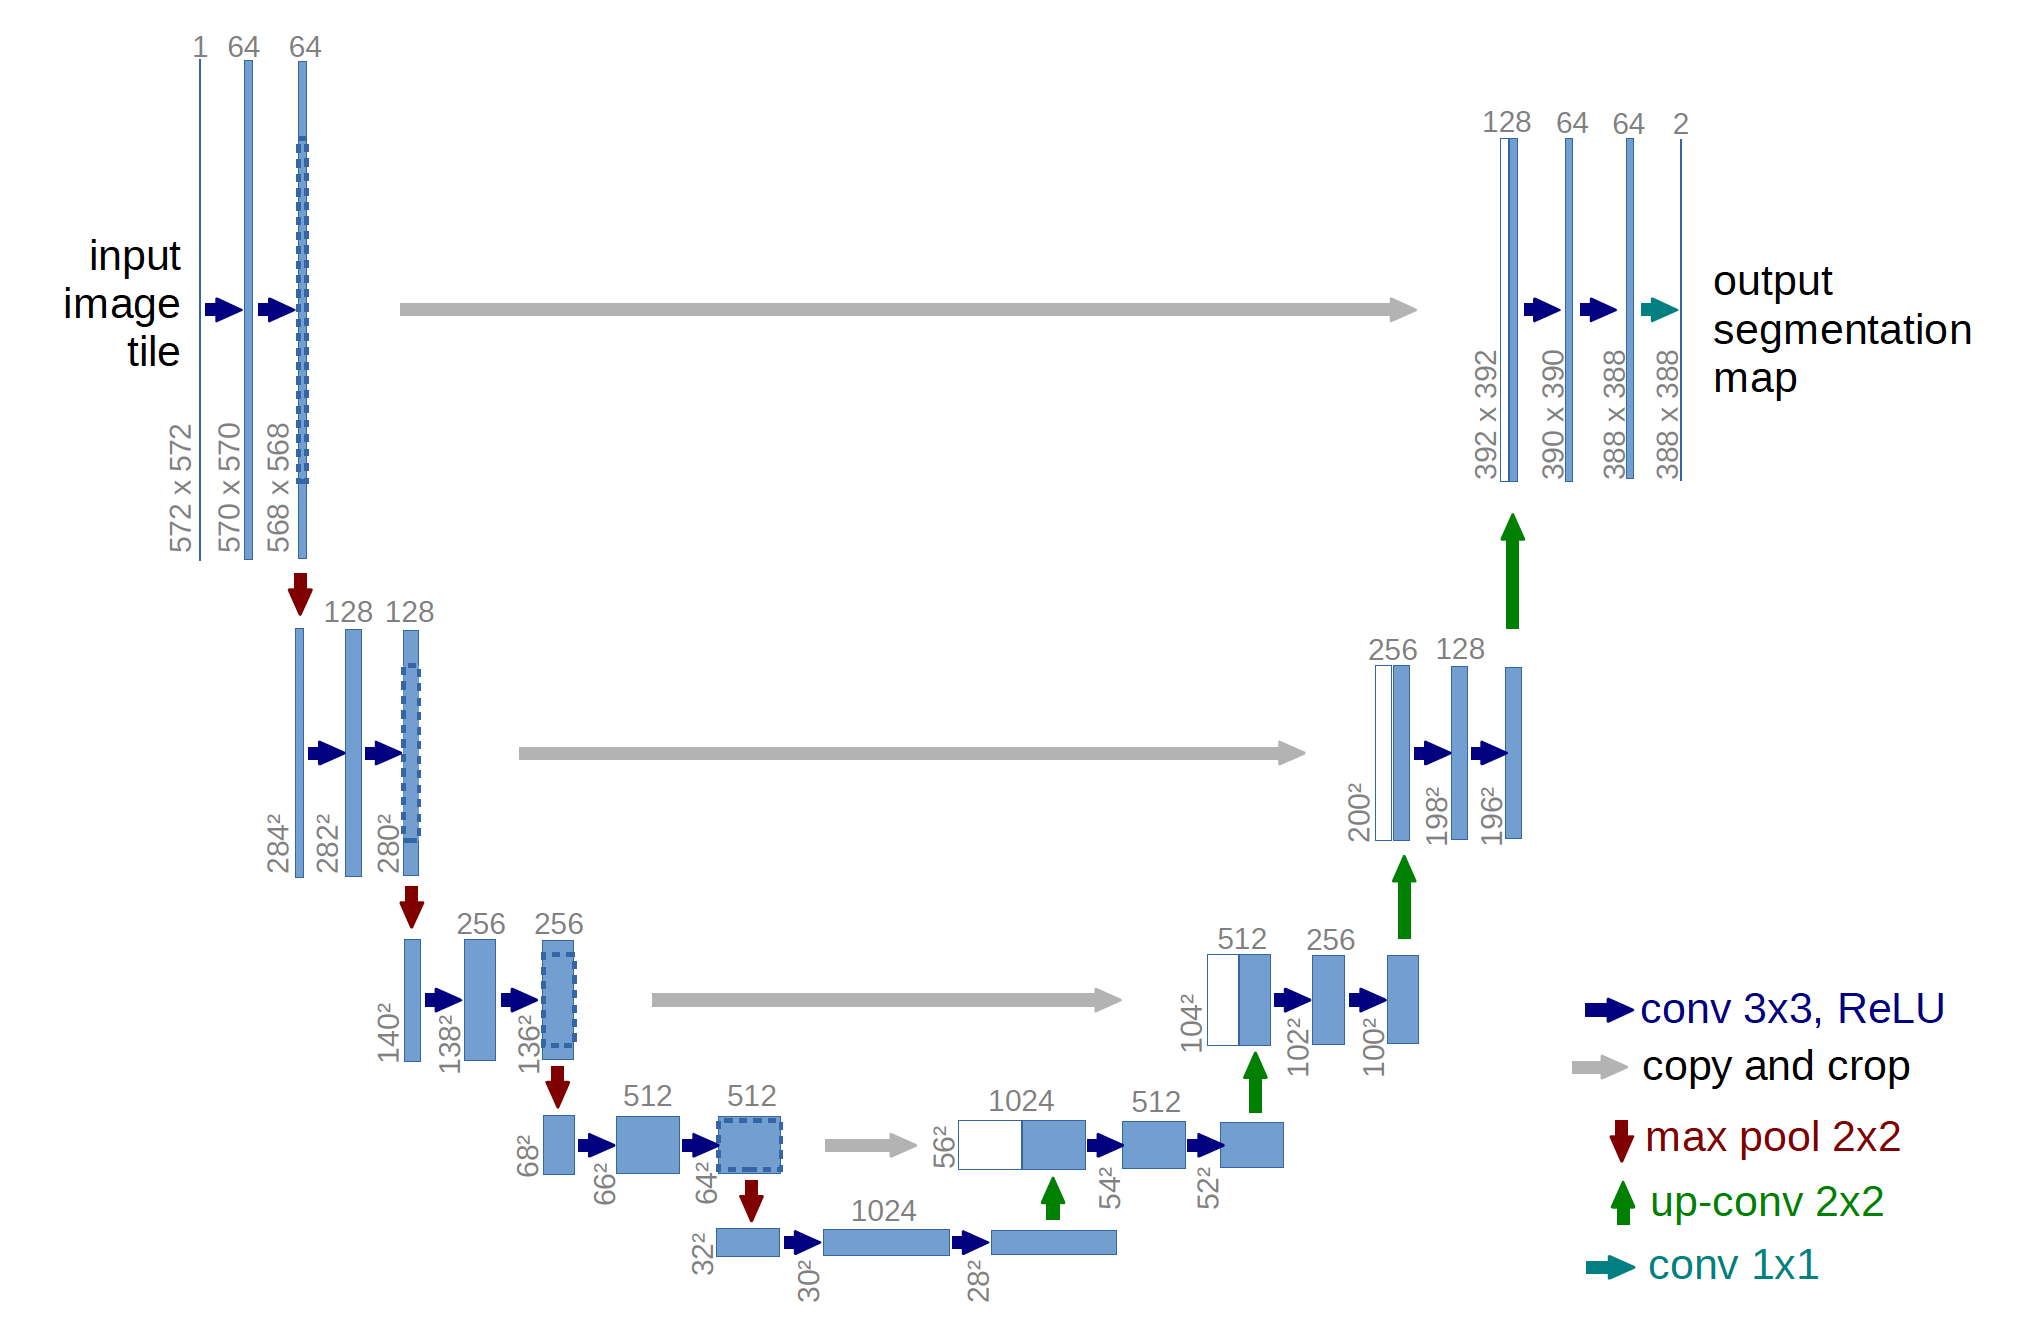
\includegraphics[width=0.8\linewidth]{chap2_Unet.png}
\end{center}
\caption{U-net架构\cite{ronneberger2015u}(最低分辨率为$32\times32$像素图片的示例)。每个蓝色矩形框对应于多通道特征图。通道数显示在矩形框顶部。 特征图的尺寸在的矩形框左下边缘。白色矩形框表示复制的特征图。箭头表示不同的操作。}
\label{fig:chap2_Unet}
\end{figure}

\textbf{空洞卷积}~
Fisher Yu 等\cite{yu2015multi} 提出了空洞卷积架构,这种结构代替了池化,一方面它可以保持空间分辨率,另外一方面它由于可以扩大感受野因而可以很好地整合上下文信息,见图\ref{fig:dilatedConv1}和\ref{fig:dilatedConv2}

\begin{figure}[h]
\begin{center}
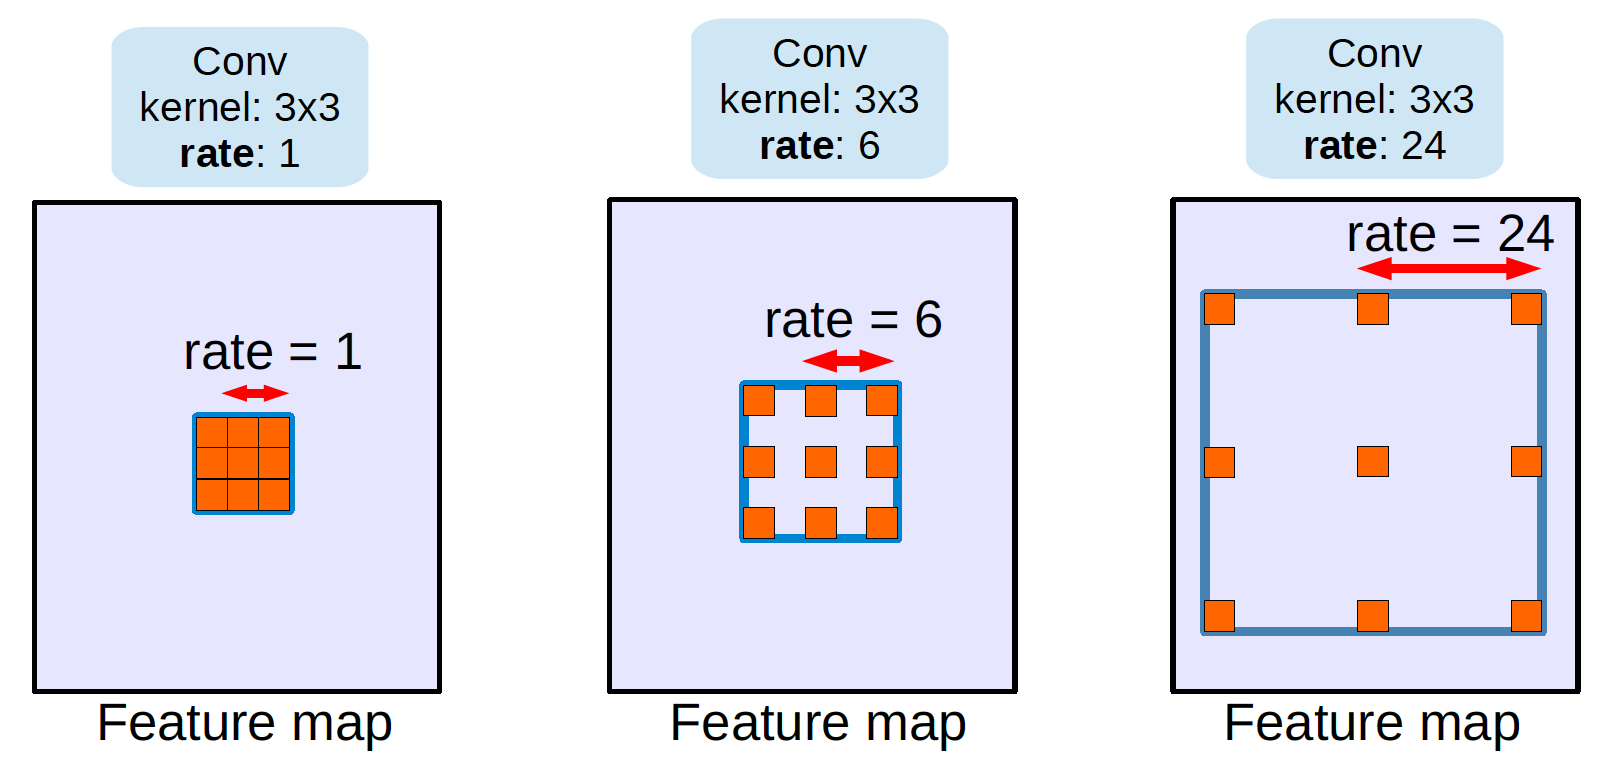
\includegraphics[width=0.7\linewidth]{diConv1.png}
\end{center}
\caption{核大小为 $3\times3$ 和不同步长的空洞卷积\cite{yu2015multi}。 标准卷积对应于步长为1。采用大的步长扩大了模型的感受野,可以在多个尺度上实现对图像编码。}
\label{fig:dilatedConv1}
\end{figure}

\begin{figure}[h]
\begin{center}
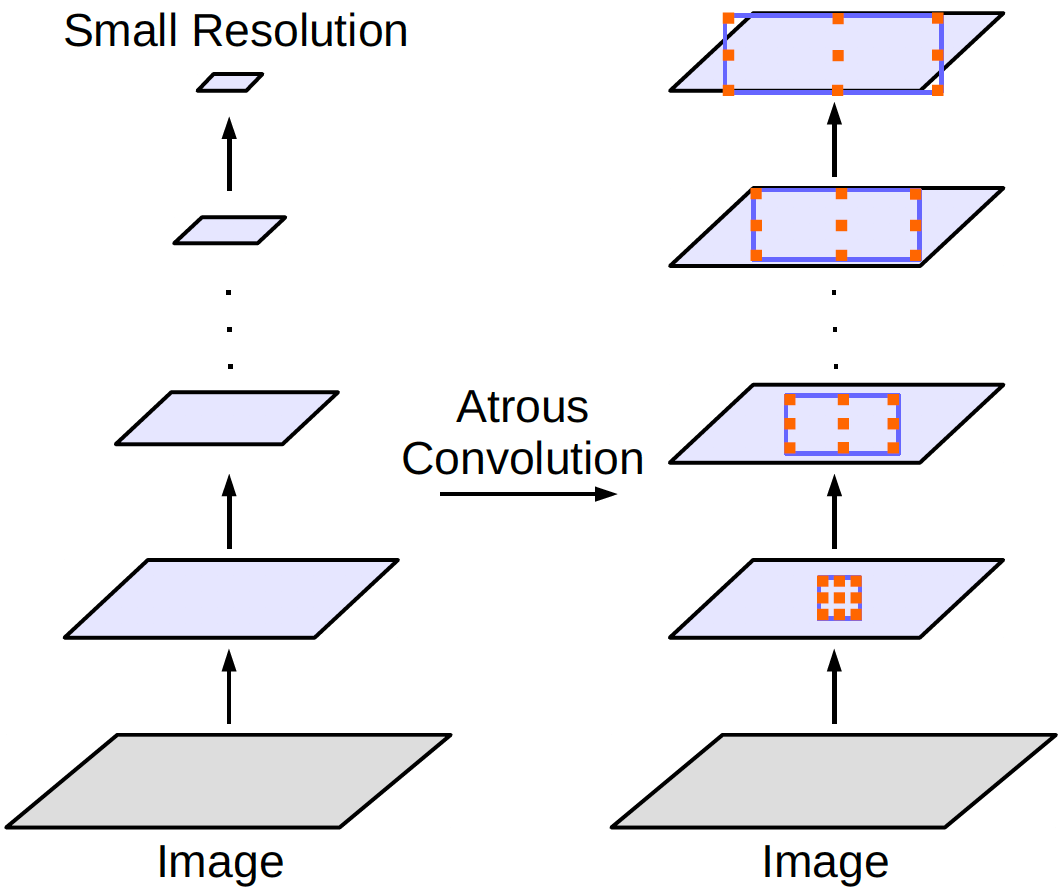
\includegraphics[width=0.5\linewidth]{diConv2.png}
\end{center}
\caption{使用空洞卷积\cite{yu2015multi}进行下采样}
\label{fig:dilatedConv2}
\end{figure}


\textbf{DeepLab系列}
\cite{chen2017deeplab}
同样使用了空洞卷积结构,可以在不增加参数的情况下扩大感受野,保持分辨率,并在此基础上提出了感受野金字塔池化,用来整合多尺度信息。同时在分割后使用全连接条件随机场(fully connected CRF)进行后处理,改善分割结果。并通过两种方式来进行多尺度的处理,一是将原始图像的多种尺度送给网络进行训练,二是通过平行的不同空洞率的空洞卷积层来获得。

\begin{figure}[ht]
\begin{center}
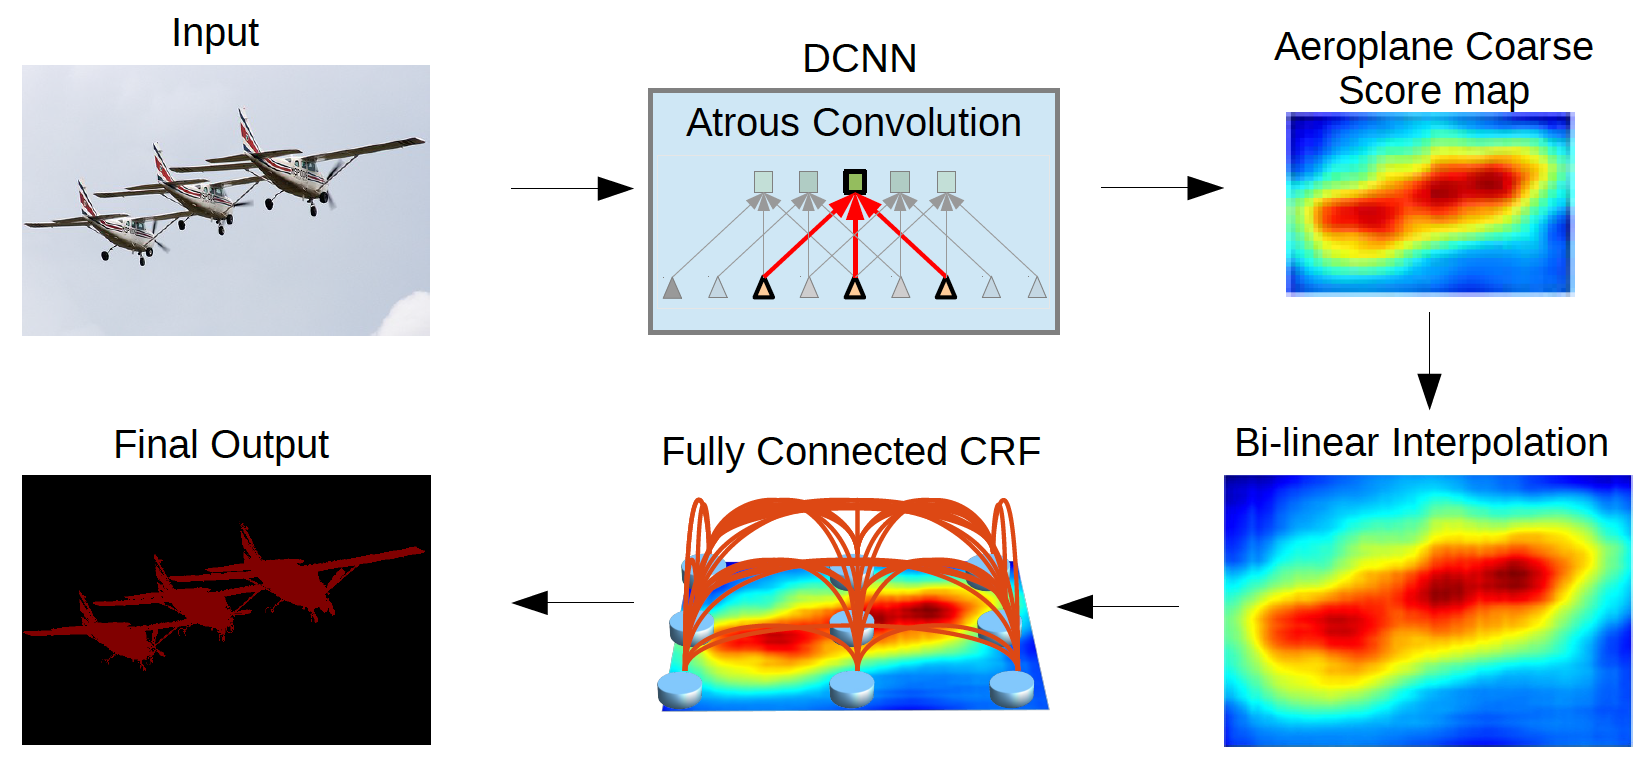
\includegraphics[width=0.8\linewidth]{DeepLab2.png}
\end{center}
\caption{DeepLab模型流程图\cite{chen2017deeplab}。 完全诸如VGG-16或ResNet-101的深度卷积神经网络卷积方式,使用空洞卷积来下。采样双线性插值将特征映射放大到原始图像分辨率。 然后采用完全连接的CRF用于细化分割结果并更好地展现对象的边界。}
\label{fig:DeepLab2}
\end{figure}

\begin{figure}[ht]
\begin{center}
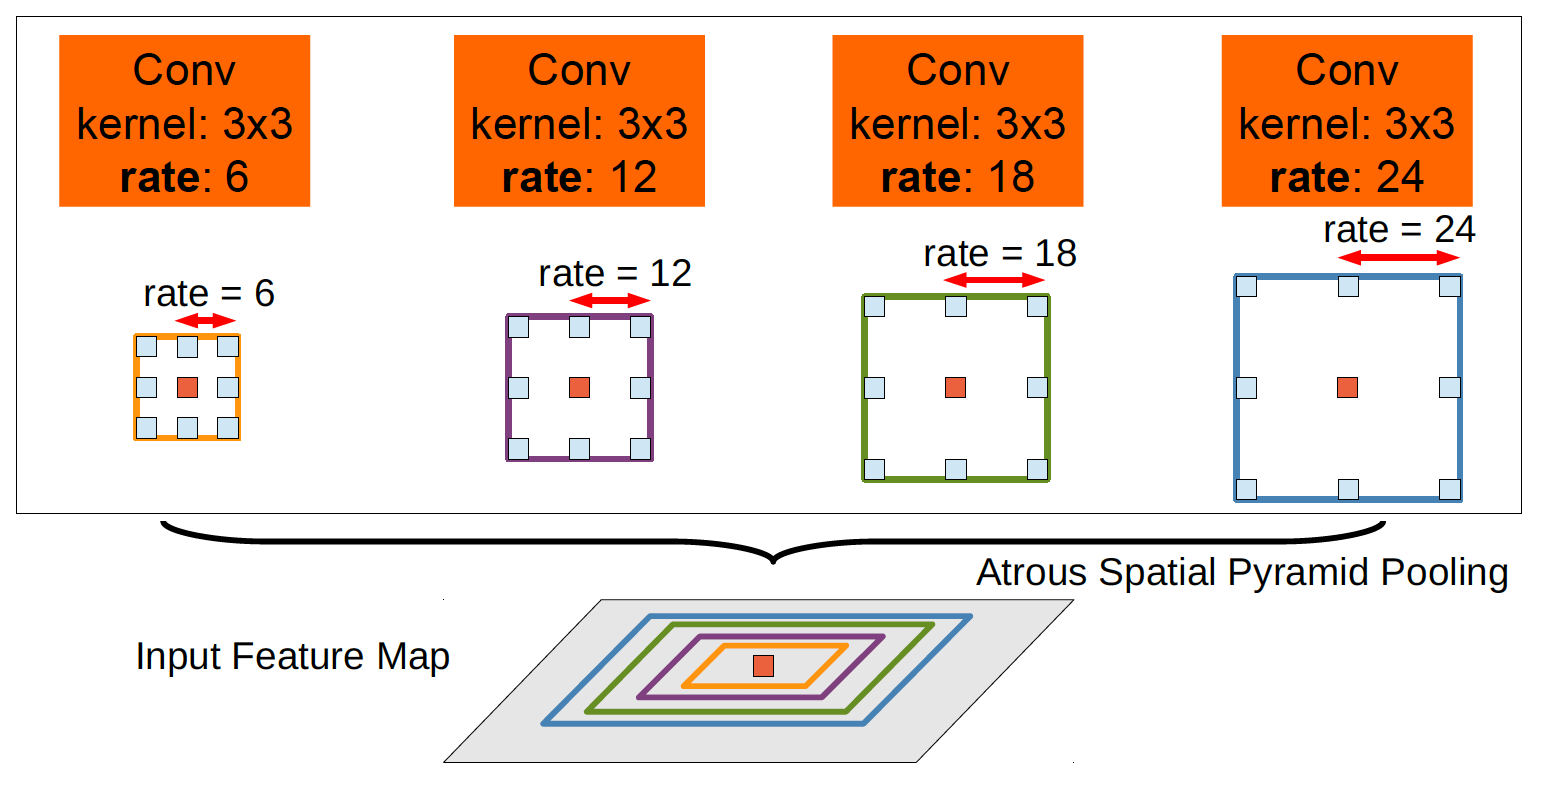
\includegraphics[width=0.8\linewidth]{DeepLab1.png}
\end{center}
\caption{空洞卷积金字塔池化\cite{chen2017deeplab}。 为对中心橙色像素进行分类,ASPP利用了多尺度并行的空洞卷积操作。}
\label{fig:DeepLab1}
\end{figure}

因为空洞卷积方法应用于语义分割也是有缺点的,即使用了大分辨率的特征图,因此计算代价大,并且需要大量的内存,于是Guosheng Lin等在2017年提出了RefineNet\cite{lin2017refinenet}。RefineNet使用编码器-解码器架构。编码器部分使用RESNET-101。解码器部分具有RefineNet 结构,它将此前解码器的低分辨率特征和编码器部分高分辨率特征进行叠加,见图\ref{fig:RefineNet1}。
\begin{figure}[ht]
\begin{center}
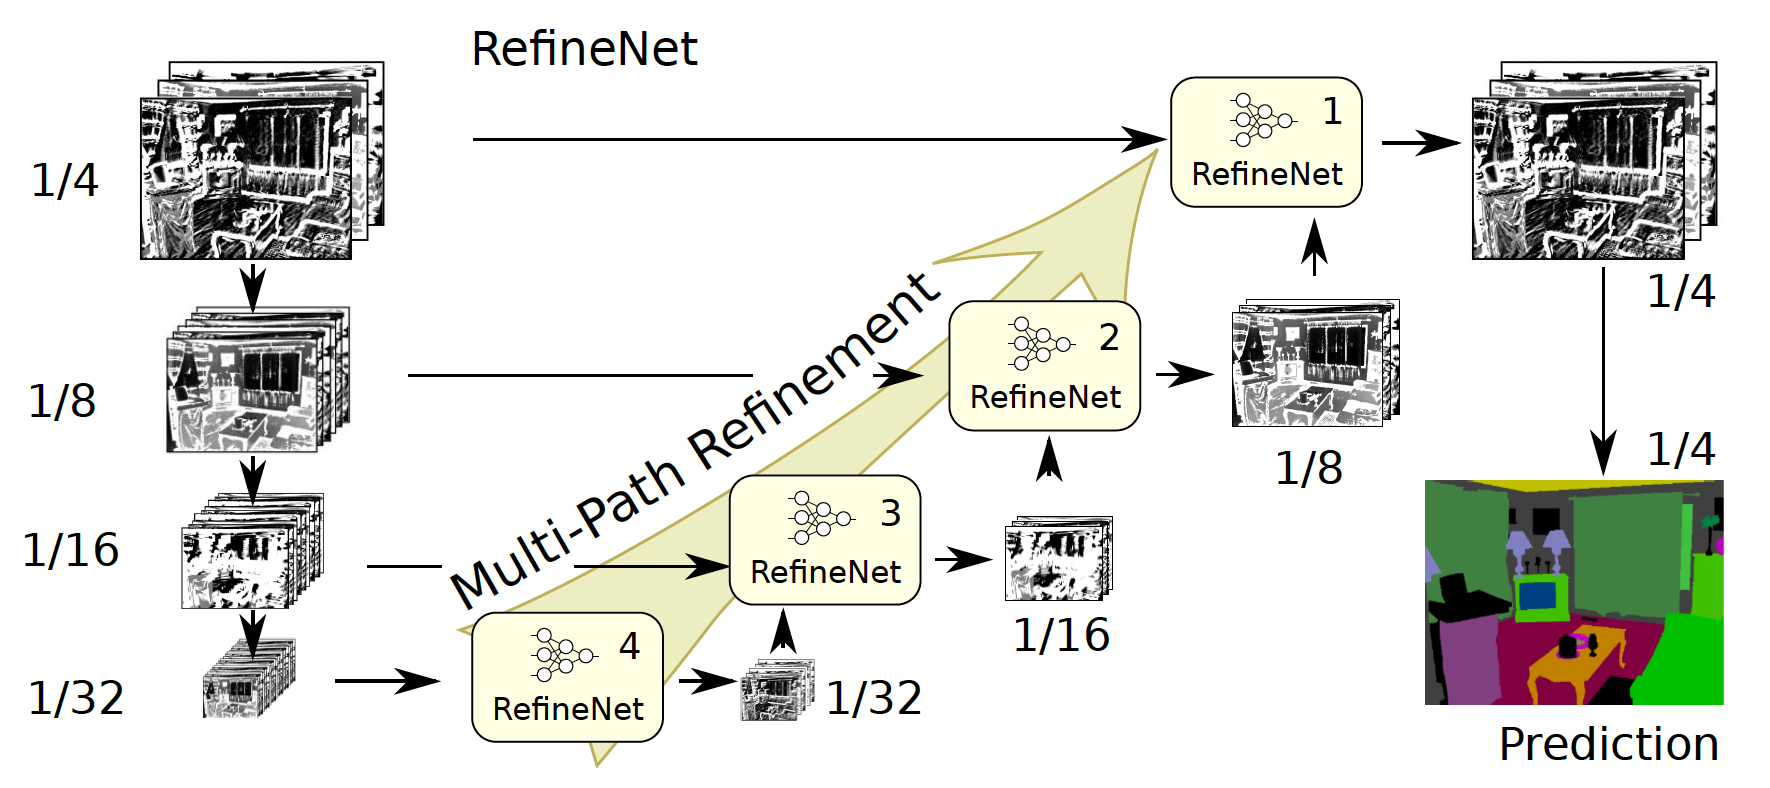
\includegraphics[width=0.8\linewidth]{RefineNet1.png}
\end{center}
\caption{RefineNet架构\cite{lin2017refinenet}。 在卷积的不同阶段利用各种层次的细节,并将它们融合以获得高分辨率的分割图,无需保存或者计算中间过程的特征图。}
\label{fig:RefineNet1}
\end{figure}

\section{弱监督分割相关研究}

由于语义分割训练需要对图像中的每一个像素进行标注,导致标注数据非常耗时,其复杂程度远远超过图像分类、目标检测。想要训练一个分割模型往往需要耗费大量的人力在掩模图像的标注上。为了解决这一问题,人们探究用 图像级别的分类标签、检测标签或者Scribble这样比较容易的标注来训练语义分割模型,这就是弱监督语义分割。通过调研近些年弱监督领域的论文,其基本思想具有下面三个特点:
\begin{enumerate}
\item 大多使用类激活图获取最特别的响应区域,作为最初始的种子类别,然后通过扩张种子区域的方式完成分割。
\item 大多与传统算法相结合。由于深度学习的分割只是看高层语义之间的一致性,没有考虑位置与颜色等低级别一致性,在做相似度度量的时候往往无法满足要求。
\item 流程目前大多还都比较繁琐,一般都需要多次扩充和更新监督信息,进行多轮训练。
\end{enumerate}

在2018年,Yunchao Wei 等\cite{wei2018revisiting} 的主体思路是利用在ImageNet上预训练的分类模型加上不同扩张率的空洞卷积,在图像上得到响应图定位物体,通过阈值分割之后用在类激活图上选择响应较大的区域,将其作为监督来训练网络。其优势在于把空洞卷积使用于分类网络,并且通过改变卷积的扩张率控制热图响应的稀疏程度。

\begin{figure}[ht]
\begin{center}
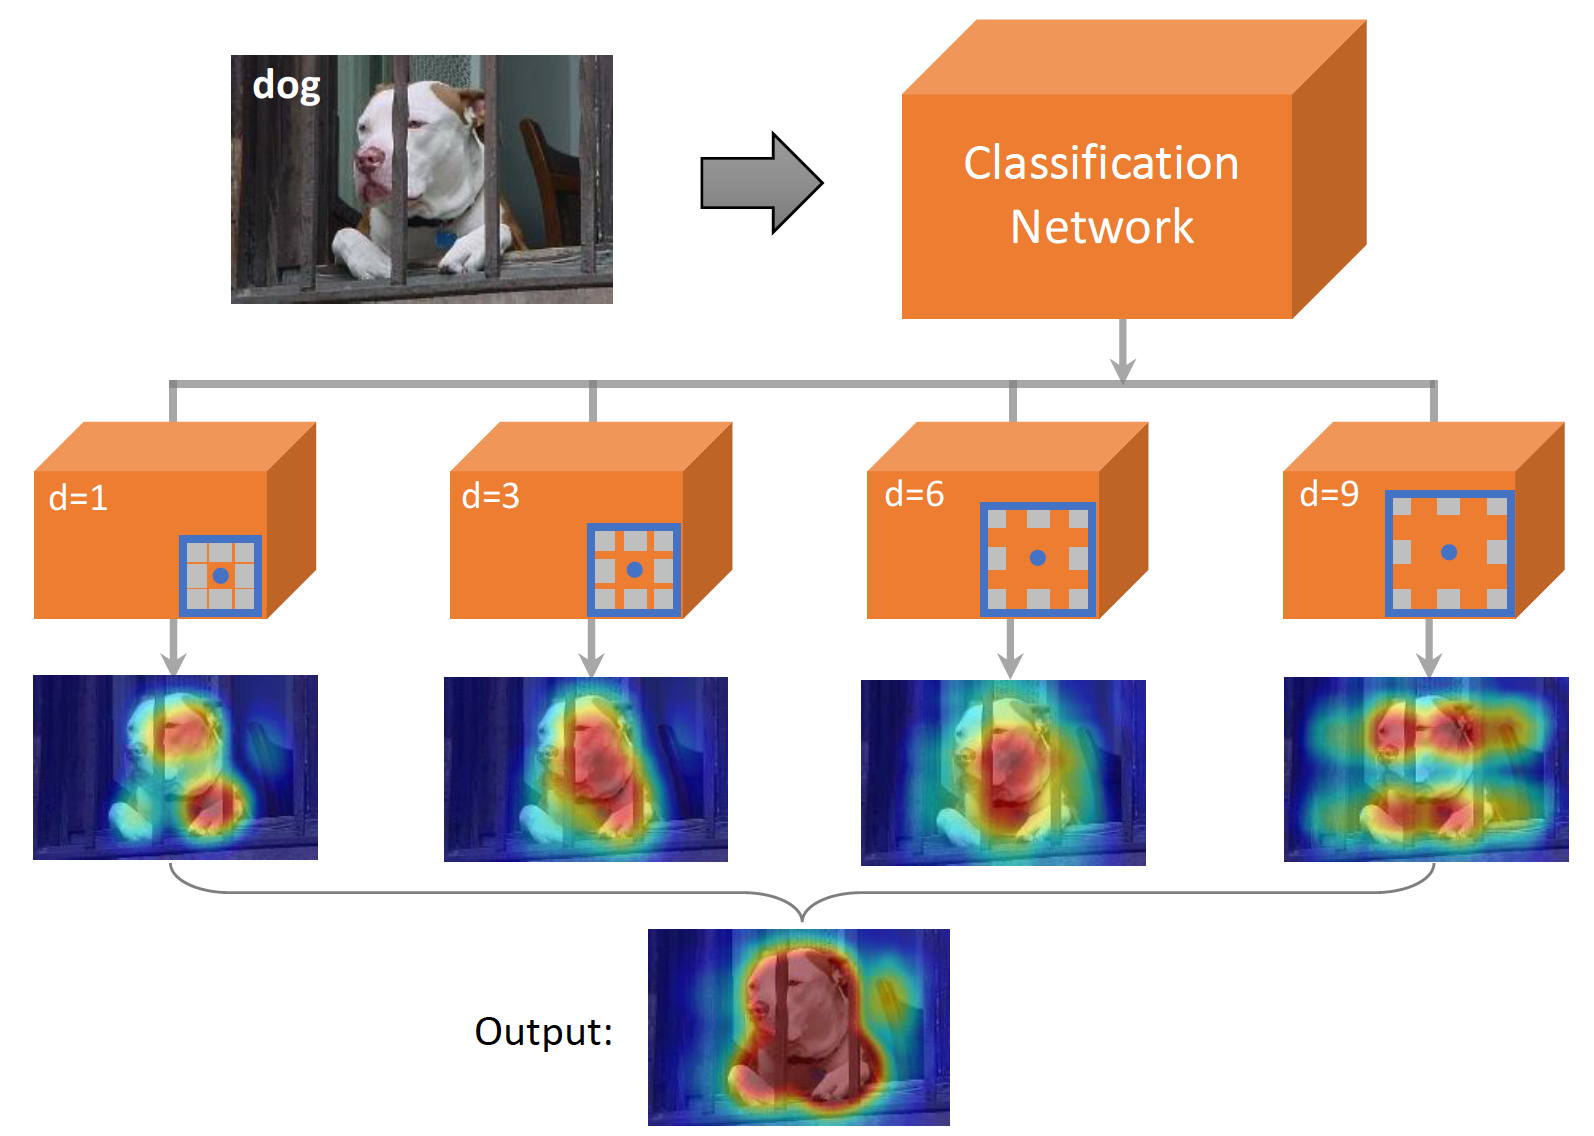
\includegraphics[width=0.6\linewidth]{dilatedConvWeaklySupervised1.png}
\end{center}
\caption{通过多种尺度的空洞卷积生成类激活图\cite{wei2018revisiting}}
\label{fig:dilatedConvWeaklySupervised1}
\end{figure}

\begin{figure}[ht]
\begin{center}
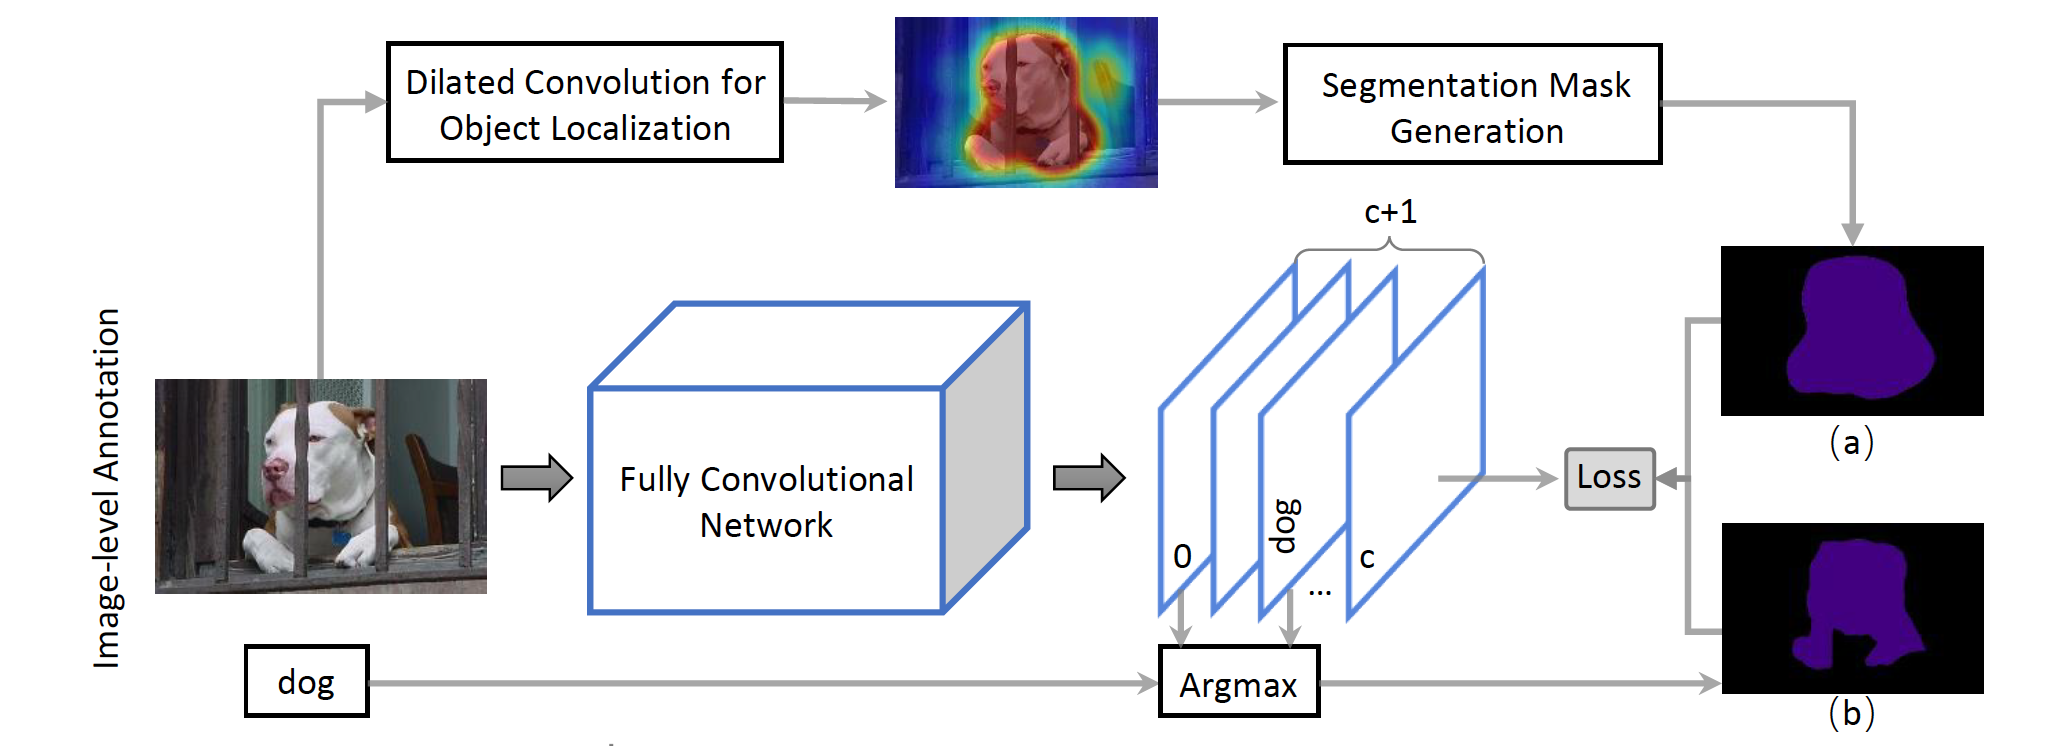
\includegraphics[width=\linewidth]{dilatedConvWeaklySupervised2.png}
\end{center}
\caption{训练流程\cite{wei2018revisiting}。使用生成的类激活图作为监督。}
\label{fig:dilatedConvWeaklySupervised2}
\end{figure}

如图\ref{fig:dilatedConvWeaklySupervised1} 中 $d = 1$所示,热图响应的问题在于只能找到一些具有判别性的稀疏区域,而物体的很多特征不明显的区域会被忽略,而用扩张率较大的空洞卷积可以得到较大的响应区域。 采用如下公式把得到的响应加权以得到较好的预测结果。
\begin{equation}
H=H_{0}+\frac{1}{n_{d}} \sum_{i=1}^{n_{d}} H_{i}
\end{equation}
$H_{0}$代表 $d = 1$的结果,$n_d$就是不同扩张率卷积的个数。整个网络做弱监督的训练流程就如图\ref{fig:dilatedConvWeaklySupervised2}所示,使用多扩张率空洞卷积网络从图像级的标注变为粗糙的预测(a),然后把(a)用作分割的监督信息。

同样在2018年,Xiang Wang等\cite{wang2018weakly}也是用分类网络的热图响应作为起始种子,之后采用迭代的方法,训练两个网络:RegionNet 和 PixelNet,令该两个网络的预测交替成为对方的监督标签,多轮迭代之后,两个网络的预测结果都逐步提升,测试时就使用训练好的PixelNet做单次预测。

由于起始种子部分仅仅覆盖了的很小局部,所以训练出来的RegionNet的结果也会遗漏很多区域,直接做监督效果不好。所以加入了Saliency-guided Refinement模块,相当于使用显著性检测的结果扩充RegionNet的输出。 区别于逆向擦除方法,这里不断更新RegionNet的结果来当做PixelNet的监督,使得预测错误的标签有不断修正的可能。传统的方法不断的扩充标签区域当做训练样本,使得在某一步被误分类的区域一直保留在标签集中误导训练结果。
\begin{figure}[ht]
\begin{center}
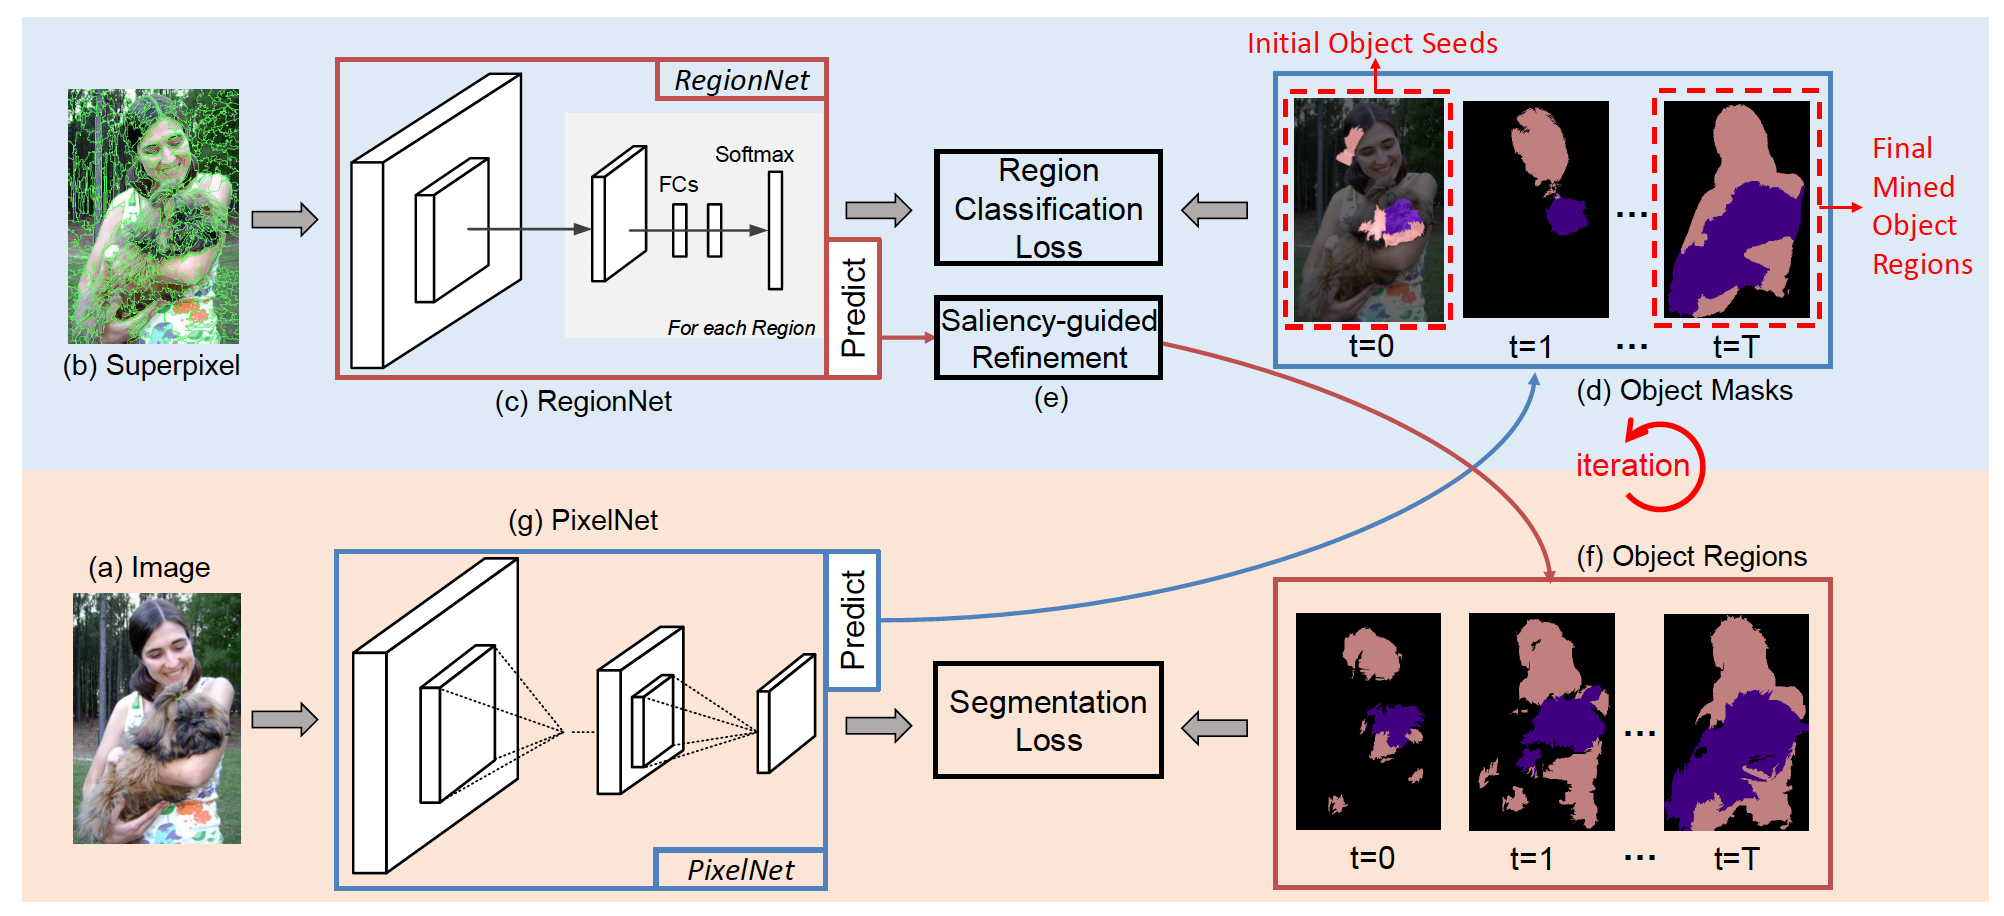
\includegraphics[width=\linewidth]{IterativelyMiningWL.png}
\end{center}
\caption{使用两个网络交替作为监督训练\cite{wang2018weakly}。对于(a),先用传统算法划分成小的区域得到(b) 超像素,然后使用预训练的分类模型在(b)上得出类激活图,取响应最高的部分作为起始种子,如右上角$t = 0$的情况。然后以得到的初始种子点作为监督训练RegionNet。把RegionNet的结果当做监督训练PixelNet。把PixelNet的预测结果当做监督训练RegionNet。不断地重复上述过程。}
\label{fig:IterativelyMiningWL}
\end{figure}


同样在2018年,Zilong Huang等\cite{huang2018weakly}的主体思路是利用预训练好的分类网络在图像上得到类激活图,用最据判别性的小区域作为起始的种子点, 然后改进传统的区域生长方法,使得被标记的区域从起始的小区域不断扩充,在训练过程中逐步得到更多的监督区域。与\cite{wang2018weakly}不同的是起始区域的扩张方法和训练所用的代价函数。这篇文章中,训练的代价函数分为种子代价和边界代价,分别用于约束区域与边界。扩张方法利用的是网络输出的结果。在语义特征层面计算像素之间的相似度,在已经有标签区域的相邻像素点计算和各个类别的相似度,相似度大于某一个阈值就把相邻点扩充进预测概率最大的那一个类别。所以,随着训练次数的增多,已标注区域区域会越填越满,提供的监督信息也会越来越多。

但其缺点是,使用区域生长方法得到的监督无法剔除被标错的区域。也就是说如果一开始有扩充错的区域,那么该区域就不会再接下来的训练中被更正。
\begin{figure}[htbp]
\begin{center}
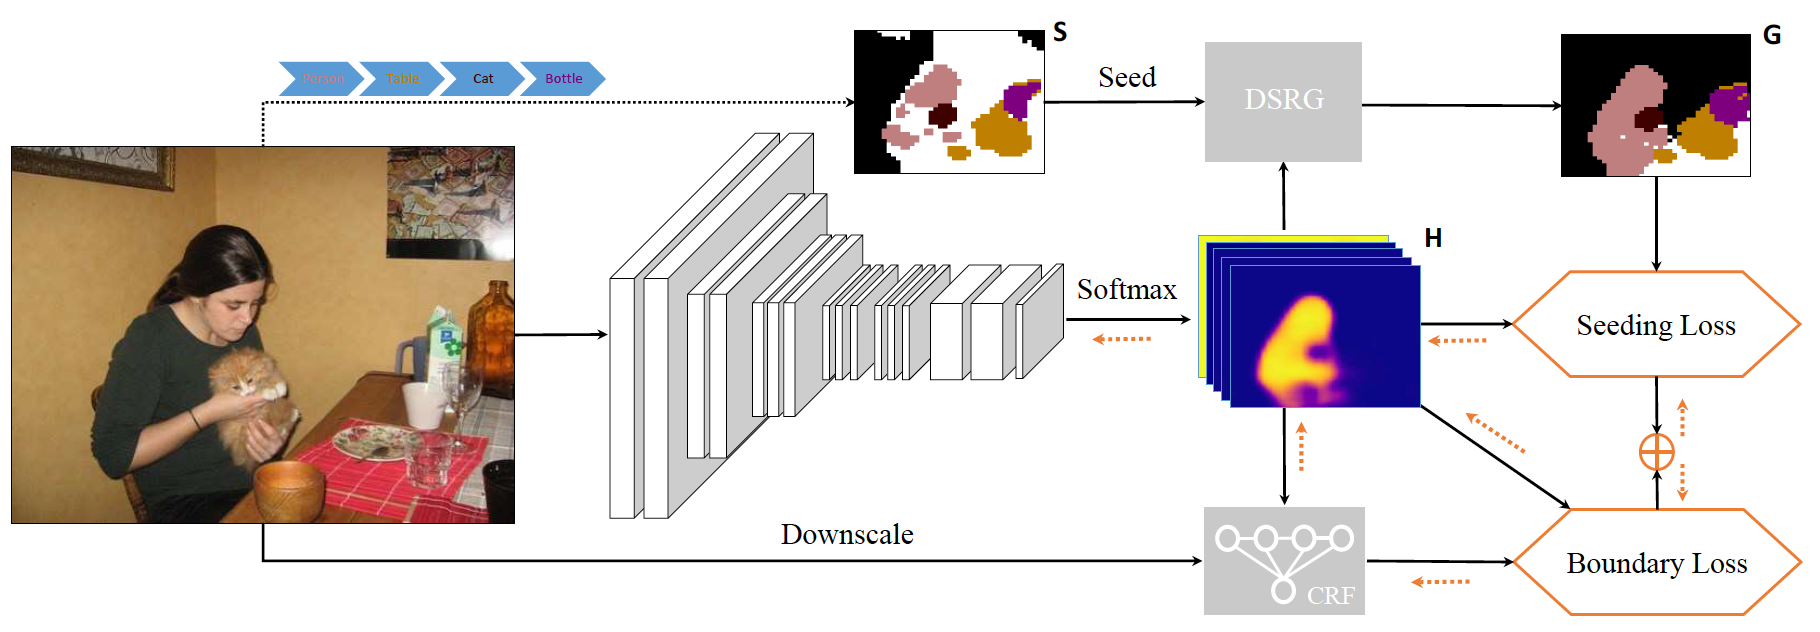
\includegraphics[width=\linewidth]{RegionGrowingWL.png}
\end{center}
\caption{使用类激活图确定种子区域,然后使用区域生长方式扩充区域,同时结合区域代价与边界代价对网络进行训练\cite{huang2018weakly}。}
\label{fig:RegionGrowingWL}
\end{figure}

Yanzhao Zhou等\cite{zhou2018weakly}同样在2018年发表了其关于弱监督下的实例分割方法,据本文作者所知,应该这是第一篇将弱监督用于实例分割任务的工作。其思路非常新颖: 先训练一个网络,使得网络响应的局部极大值可以指示每一个实例物体所在的位置,然后用这些局部极大值的点反向传播信息,逐层向前找到每层网络与那些极大值点相对应的区域,得到峰值响应图 (Peak Response Map), 之后结合峰值响应图以及其提供的边界、位置、类别信息,结合现有的一些传统算法,提出局部的掩模,然后通过非极大抑制 (NMS)得到较为精细的实例分割结果。

由于类激活图的峰值代表图片中某个类别最据判别性的部分,但是不一定可以代表每一个实例的位置。于是,这篇文章首先训练一个网络使得类激活图的局部峰值可以对应每一个实例的位置,如\ref{fig:PRM1}蓝色区域所示。
\begin{figure}[htbp]
\begin{center}
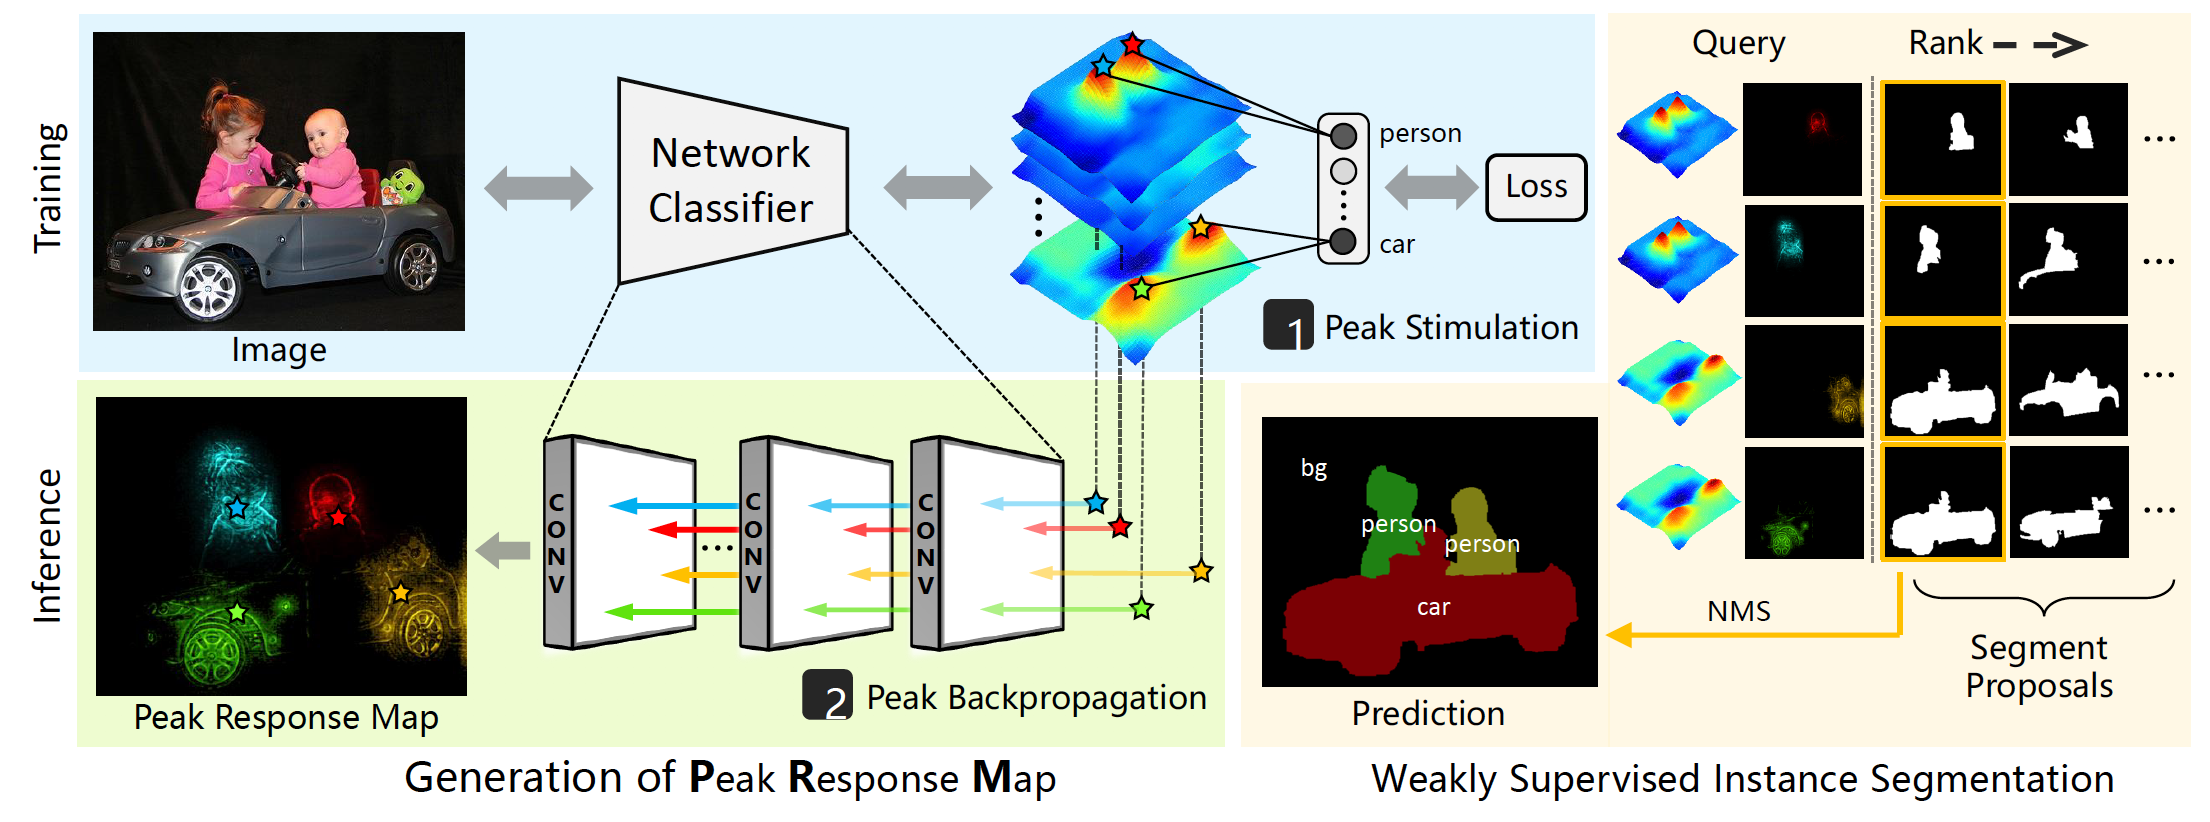
\includegraphics[width=\linewidth]{PRM1.png}
\end{center}
\caption{峰值响应图的生成过程\cite{zhou2018weakly}}
\label{fig:PRM1}
\end{figure}

值得注意的是,在训练时作者先用了一个Dirac函数在类激活图上卷积,目的是只提取峰值区域,这是因为只有峰值的那几个点是想要的有效区域(正样本),其他的大块区域都是并不代表实例的负样本,如果不把峰值区域提取出来,这少数的几个点所提供的正样本的梯度就会淹没在大量的负样本之中。在推理的时候,作者先用训练好的网络找到代表每一个实例位置的峰值点,然后通过反向传播计算这些峰值点来自于前一层每个点的概率,这样一层一层向前推算,就得到第一层的峰值响应图, 如图\ref{fig:PRM2}所示。 得到了峰值响应图之后,利用各种传统算法预测出来局部掩模,最后利用峰值响应图的信息和类别信息进行筛选,然后再这些掩模之中进行非极大抑制 (NMS) 即可。

\begin{figure}[htbp]
\begin{center}
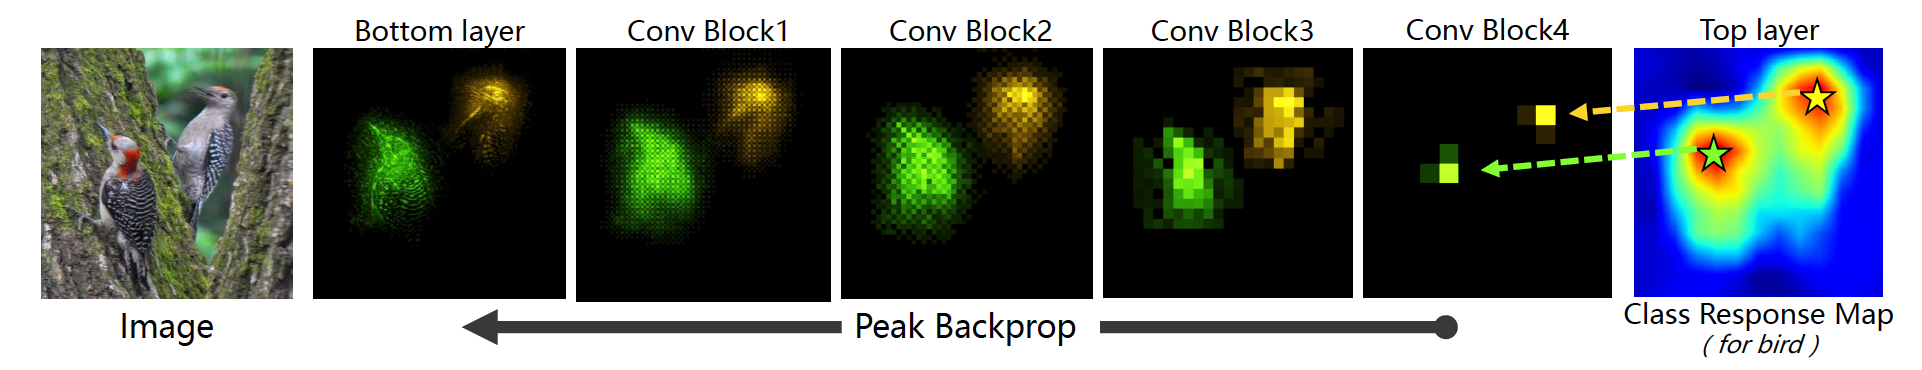
\includegraphics[width=\linewidth]{PRM2.png}
\end{center}
\caption{峰值响应反向传播过程\cite{zhou2018weakly}}
\label{fig:PRM2}
\end{figure}

近几年来,还有一些弱监督分割的方法。例如,通过涂鸦\cite {lin2016scribblesup, xu2015learning}和物体边界框\cite {dai2015boxsup}对图像进分割。然而,这些方法仍然需要大量的人力。一些研究使用图模型来推断区域的标签\cite {zhang2015weakly, lai2016saliency},但他们的对物体的检测能力仍然难以尽如人意。有些方法\cite {papandreou2015weakly, bearman2016s, wei2016learning}试图通过使用可以对位置提出猜测的探测器来定位对象\cite {arbelaez2014multiscale, cheng2014bing}。然而,由于探测器使用边界框标注或对象边界标注进行训练,因此仍需要大量人力。

相反,在本文的工作中,基于类激活图\cite{zhou2018weakly,huang2018weakly}的思想,使用标准分类网络来生成具有卷积响应的类感知激活图,然后结合基于超像素上所建立的图模型,再通过显著性传播实现分割,在此框架中,白癜风区域的边界得到很好的保留。
\section{超像素分割}\label{sec:SLIC}
\subsection{方法原理}
Achanta等\cite{achanta2012slic}提出了一种简单而优雅的迭代聚类算法 (SLIC),用于将彩色图像分割成超像素。该方法的主要思想便是把一些具有相似特性的像素“聚合”起来,形成一个更具有代表性的大“元素”。而这个新的元素,将作为其他图像处理算法的基本单位。将超像素分割用于白癜风分割任务有三个好处:
\begin{enumerate}
\item 大大降低了维度。使用超像素作为后续算法的输入,可以很大程度上减少后续算法的计算量,提高速度。
\item 可以剔除一些异常像素点。由于在白癜风分割的任务中,图片没有经过精细的校准和增强,且拍摄物体多样,因此,对于噪声或者较小区域的异常点可以通过超像素来剔除。
\item 保留较完整准确的皮损边界。经过实验发现,超像素对皮损边界非常的敏感,因此本文利用这一点,将超像素分割作为弱监督分割方法的预处理。
\end{enumerate}

但是由于输入图像的大小差别很大,如何确定初始种子点数目成为了一个难点,如果初始化种子点数目过多,则既没有办法降低数据维度,也没有达到剔除一些异常像素点的目的;如果初始化种子点数目过少,则没有办法很精确的捕捉皮损边界,这样对之后的弱监督分割方法的效果会产生影响。因此,基于原方法,本文通过自适应地调整超像素的数量,来满足预处理的要求:
\begin{equation}
\label{eq:Nc}
N_{c}=\left(\frac{W}{\rho}-1\right)\left(\frac{H}{\rho}-1\right)
\end{equation}
其中,$N_c$为聚类种子点个数,$W$与$H$分别为图像的宽度和高度,ρ此处定义为种子点密度,取值范围为$[0,min⁡(W,H)]$,实验中取为$20$,可以根据需要设置$\rho$的值。$\rho$越大,种子点越密集,后期得到的每个聚类中心面积就越小,分割越细致,但过大的密度会增加计算量,并且容易受到图像噪声的干扰,导致图像分割效果变差。

\begin{figure}[htbp]
\begin{center}
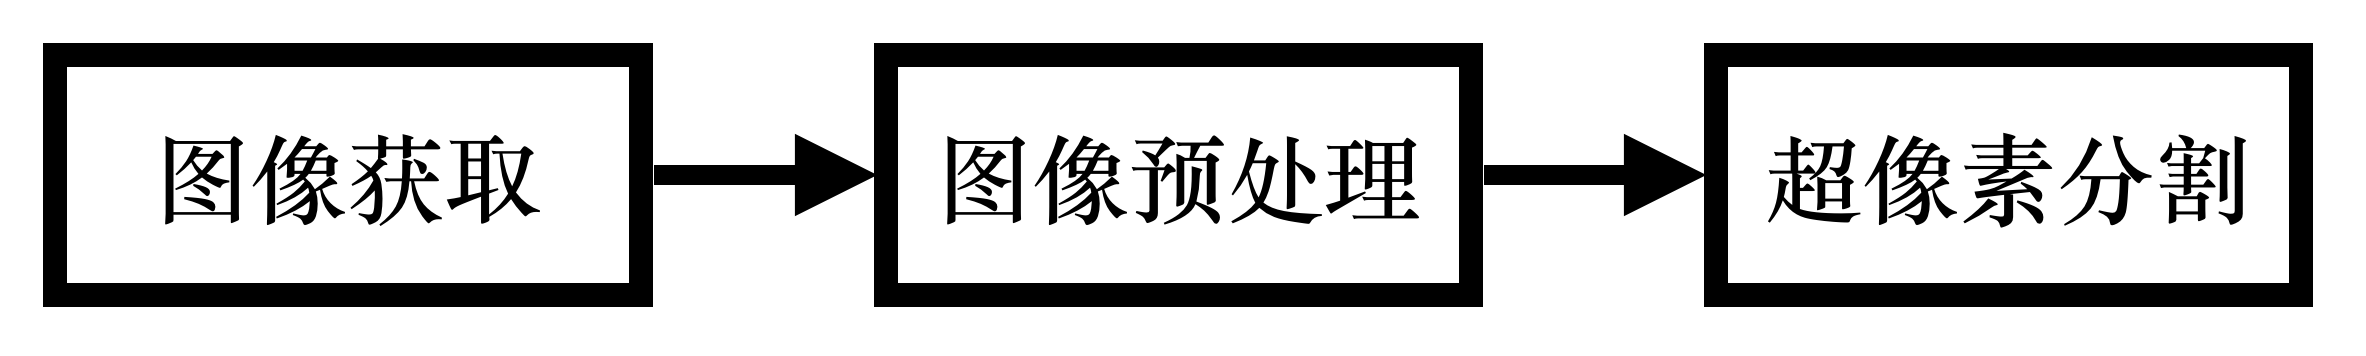
\includegraphics[height=1.5cm]{chap3_superpixelflow.png}
\end{center}
\caption{超像素分割实验流程图}
\label{fig:chap3_superpixelflow}
\end{figure}

\textbf{图像获取}:可使用手机、相机、专业医疗设备对患处拍摄图片,皮肤应占据照片的主体部分,但仍可包含部分背景、衣物、毛发等无关的区域,拍摄时应尽量选择光线较为柔和的环境。在实验部分的测试图片选用Vit2019中的图片作为测试。

\textbf{图像预处理}:此步骤的目的一是为了去除噪声,二是平滑毛发区域中的锐利边缘,避免聚类中心分割时产生过多的不规则形状以及孔洞。对图像使用了高斯模糊和中值滤波来去除噪声。

\textbf{超像素分割}:此部分将有相似特性的像素聚合起来形成超像素。具体算法流程见算法2。
\begin{table}[htbp]
  \centering
    \begin{tabular}{l}
    \toprule
    \textbf{算法2}  改进的超像素分割算法流程\\
    \midrule
    \multicolumn{1}{p{36em}}{1. 将输入RGB图像转换到Lab颜色空间} \\
    2. 根据输入图像尺寸初始化聚类种子点个数,见公式(\ref{eq:Nc})\\
    \multicolumn{1}{p{36em}}{3. 以$\rho$为步长,初始化种子点,记为$\mathrm{C}_{\mathrm{k}}=\left[l_{k}, a_{k}, b_{k}, x_{k}, y_{k}\right], \quad k=1,2, \dots, N_{c}$, 其中$l_{k}, a_{k}, b_{k}$ 分别为图像在Lab空间下位置坐标为$\left(x_{k}, y_{k}\right)$处所对应像素点的L,a,b分量}\\
    \multicolumn{1}{p{36em}}{4. 在以种子点为中心,3×3为大小的领域内,将种子点移动到Lab模型中L通道梯度最小的位置,以防其落到图像边缘上或者噪声处,对后面的聚类过程产生影响。}\\
    5. \textbf{聚类}\\
    \multicolumn{1}{p{36em}}{ \hspace{2em} 5-1. 初始化每一个像素点i的标签数组$l(i)=-1$,距离数组$d(i)=\infty$,初始化最大迭代次数$N_{iter}$} \\
    \hspace{2em}5-2. 以$C_k$为中心,$2\rho \times 2\rho$大小的区域内,计算像素$i$与$C_k$的距离$D$ \\
    \hspace{2em}5-3. 若${D}<{d}({i})$,则令$d(i)=D,l(i)=k$ \\
    \hspace{2em}5-4. 判断是否遍历完所有聚类中心,若是,则继续;否则返回步骤 5-1 \\
     \hspace{2em}5-5. 更新所有聚类中心\\
     \hspace{2em}5-6. 判断是否达到最大迭代次数$N_{iter}$,若是,则结束;否则,返回步骤5-2\\
    6. 增强图像的连通性,最终生成$n$个像素聚类\\
     \bottomrule
    \end{tabular}%
\end{table}%

其中,将像素$i$与像素$j$之间的距离$D$定义为空间距离与颜色距离的加权和:
\begin{subequations}
\begin{align}
\mathrm{D}_{\mathrm{s}}&=\sqrt{\left(x_{i}-x_{j}\right)^{2}+\left(y_{i}-y_{j}\right)^{2}}\\ \vspace{1em}
\mathrm{D}_{\mathrm{c}}&=\sqrt{\left(l_{i}-l_{j}\right)^{2}+\left(a_{i}-a_{j}\right)^{2}+\left(b_{i}-b_{j}\right)^{2}}\\
\mathrm{D}&=\sqrt{\left(\frac{D_{s}}{C_{s}}\right)^{2}+\left(\frac{D_{c}}{C_{c}}\right)^{2}}
\end{align}
\label{eq:D}
\end{subequations}

其中$C_s,C_c$ 分别为空间距离与颜色距离的归一化常项。

\subsection{实验结果与分析}
经过如图\ref{fig:chap3_superpixelflow}所示流程,我们至此,即可得到分割好的$n$个图像的子区域,其中$n$等于算法2步骤6中聚类的个数,如图\ref{fig:chap3_SLICresults1}所示,由蓝色线所形成的每个最小封闭区域即为一个聚类中心。然后我们通过人为施加阈值的方式对白癜风皮损区域进行分割,得到图\ref{fig:chap3_SLICresults1}.c。

此处令公式(\ref{eq:D})中的$C_s=25,C_c=\rho$. 在使用过程中,$C_c$的取值范围可取$[1,40]$之间,该值越大,则$D_s$在距离度量中所占权重越小,则后期所得聚类中心形状越不规则,呈长条状,即难以保证空间的相关性,但对物体边缘较为灵敏,贴合度较高,容易收到噪声的干扰;反之,该值越小,则$D_s$在距离度量中所占权重越大,则后期所得聚类中心形状越规则,类似方块状,不易受到噪声的干扰,但对图像边缘较不敏感。实验中取最大迭代次数为10,可达到效果与计算代价的平衡。

\begin{figure}[htbp]
\begin{center}
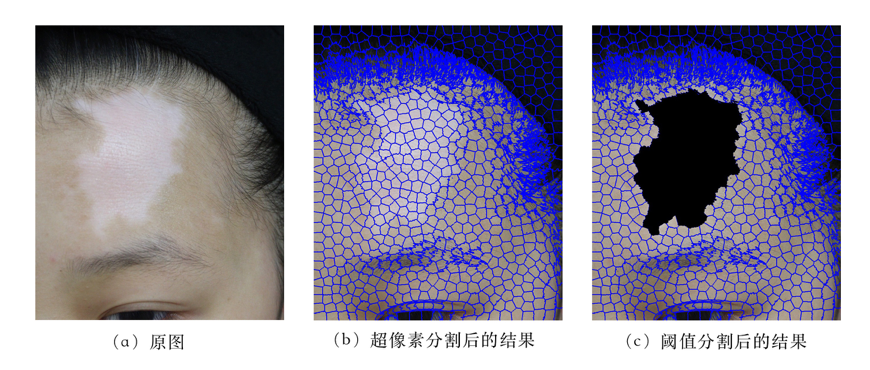
\includegraphics[width=0.9\linewidth]{chap3_SLICresult1.png}
\end{center}
\vspace{-1em}
\caption{超像素分割流程对照结果图}
\label{fig:chap3_SLICresults1}
\end{figure}

\begin{figure}[htbp]
\begin{center}
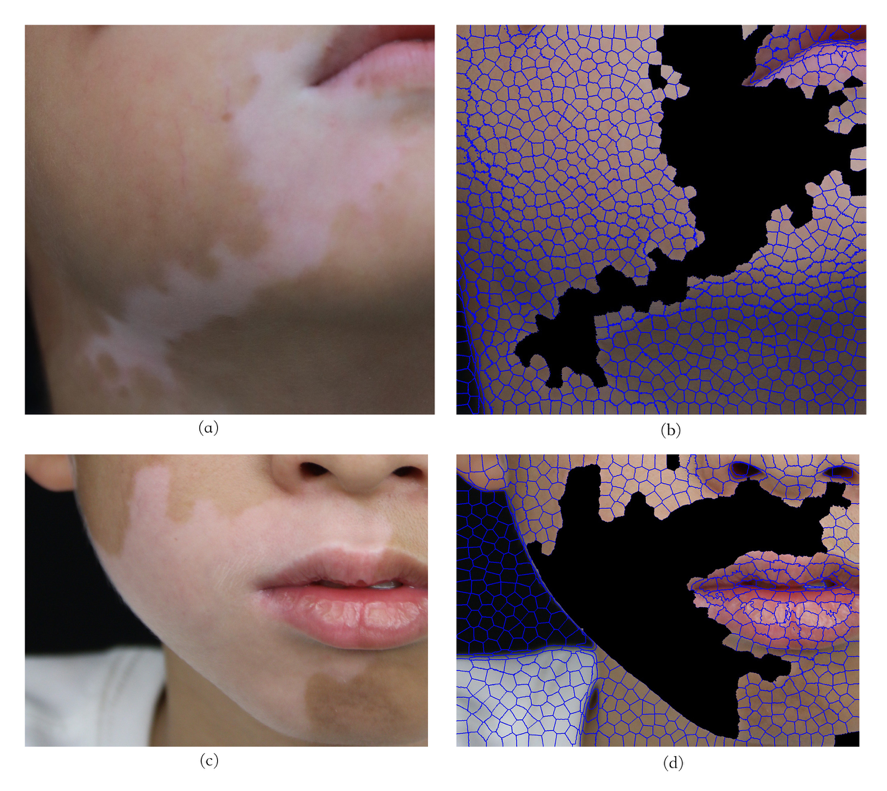
\includegraphics[width=0.6\linewidth]{chap3_SLICresult2.png}
\end{center}
\vspace{-1em}
\caption{超像素分割结果图。(a)(c)表示原图,(b)(d)表示超像素分割后的结果图。}
\label{fig:chap3_SLICresults2}
\end{figure}

通过实验可以发现,将超像素分割方法应用于白癜风图像的预处理有以下的优点:
\begin{enumerate}
\item 操作简单方便,对硬件设备没有特殊要求。
\item 可适应白斑边界模糊且图像对比度低的情况,如图~\ref{fig:chap3_SLICresults2}.a。
\item 由于引入超像素作为一块区域的代表,即便处理高分辨率图像仍可做到快速分割。算法速度可参见表\ref{table:SLICresults}
\item 分割图像不易产生空洞,不依赖于后期的形态学处理。
\end{enumerate}

\begin{table}[]
\centering
\caption{SLIC算法性能测试结果}
\begin{tabular}{cccc}
\toprule
测试图片 & 图片大小         & 运行速度(秒) & IOU  \\ \midrule
  图\ref{fig:chap3_SLICresults1}.a   & 850 × 1011   & 5.6     & 0.89 \\
    图\ref{fig:chap3_SLICresults2}.a   & 1373 × 1305 & 11.9    & 0.82 \\
    图\ref{fig:chap3_SLICresults2}.c   & 1588 × 1152 & 11.6    & 0.86 \\ \midrule
     \multicolumn{4}{c}{硬件环境:2.3 GHz Intel Core i5}\\
     \bottomrule
\end{tabular}
\label{table:SLICresults}
\end{table}

\section{本章小结}
本章首先介绍了近些年来将深度学习应用于图像分割领域的方法和技术,然后引出了基于强监督方法的缺点,即对数据集有很强的依赖性。然后本章对比了近年来各种弱监督分割方法,分析了其各自的优点和缺点,并将其基本的思想做了总结和归纳,为引出本文的弱监督分割框架进行了铺垫。

关于超像素分割部分,首先介绍了一种广泛用于图像分割领域的一种简单而优雅的迭代聚类算法 (SLIC),我们将其作为执行弱监督分割前的一项预处理步骤,并详细解释了将超像素分割用于白癜风分割任务的三个好处,即大大降低了维度、剔除一些异常像素点、保留较完整准确的皮损边界。然后指出了在经典超像素分割算法中初始种子点数目确定难的问题,并针对提出了改进的方法。最后通过实验,定性的展示了超像素分割的效果,为弱监督分割框架的介绍奠定了基础。

